\section{Exact certificates, numerical diagnostics, and reproducibility}
\label{sec:computation}

The accompanying computations have two distinct purposes. Exact
rational and finite-field calculations verify finite identities and
isolate specified algebraic numbers. High-precision quadrature and
coefficient evaluation illustrate analytic asymptotics whose proofs
are given in the preceding sections. The latter calculations do not
certify continuation of an inverse sheet or optimization over an
unbounded parameter domain.

\subsection{Finite algebra that can be replayed exactly}

The verifier \nolinkurl{code/verify_kernel_algebra.py} uses only Python's
standard library and rational arithmetic. It reconstructs the two
derivative numerators of $K_2$, computes their Sylvester resultant,
checks the elimination substitutions, obtains the primitive polynomial
for $M_2$, and proves its irreducibility modulo five. It also checks
the rational interior sample and isolates the relevant roots. Its
outward rational interval calculations certify
\begin{gather*}
 1.1189386859610526747774667909001084300609
       <M_2,\\
 M_2<1.1189386859610526747774667909001084300610.
\end{gather*}
The full rational endpoints, rather than only their decimal displays,
are retained in \nolinkurl{data/kernel_algebra.json}.

The independent verifier \nolinkurl{code/verify_cohen_c1.py} also uses
only standard-library rational polynomial arithmetic. It verifies the
exact coefficient-extraction moments through the order needed for the
first two largest-root corrections, performs the perturbation algebra,
and checks cancellation of the Euler-constant variable. The zeta-value
formula is obtained by exact substitution and
$\zeta(4)=\tfrac25\zeta(2)^2$, not by an integer-relation fit.
The record is \nolinkurl{data/cohen_c1_certificate.json}.

Two further checks compare independently generated polynomial formulas.
\nolinkurl{code/verify_diagonal_inverse.py} compares the exact Stirling
and nonlinear inverse-series recurrences through degree 35, and uses
rational enclosures of $\log2$ to certify the corresponding finite
signs. \nolinkurl{code/verify_cohen_edges.py} checks the generalized
operator normalization for $1\leq n\leq14$, $1\leq k\leq5$ and
symbolically verifies the general first coefficient $C_{j,1}$.
These finite checks are useful independent replays; the all-index
identities and asymptotic results have separate proofs.

\subsection{Large-index axis diagnostics}

Direct gamma quadrature evaluates $R_N(0,b)-1$ without subtracting
large finite Euler sums. The implementation forms
\[
 \exp\!\left(\log(1+v)+(N-1)\log(1-v^2)-\log(1+v^2)\right)-1
\]
with stable logarithm and exponential differences, then integrates
against the gamma density. The maximizing order is found by the
gamma-score derivative; negative curvature is checked numerically.
The sample below uses 65 decimal digits of working precision.

\begin{table}[htbp]
\centering
\begin{tabular}{rrr}
\toprule
$N$ & Axis maximizing $b_N$ &
$\bigl(C_N^{\mathrm{ax}}-1\bigr)/(cN^{-p})$\\
\midrule
$10^2$ & 12.3318927895 & 1.0759792475\\
$10^4$ & 23.7920662690 & 1.0296132033\\
$10^6$ & 35.1917432654 & 1.0086616486\\
$10^8$ & 46.5618035683 & 1.0025176685\\
\bottomrule
\end{tabular}
\caption{Numerical axis diagnostics. The finite numbers are not used
to choose an unproved onset threshold for global axis reduction.}
\label{tab:axis-diagnostics}
\end{table}

\begin{figure}[htbp]
\centering
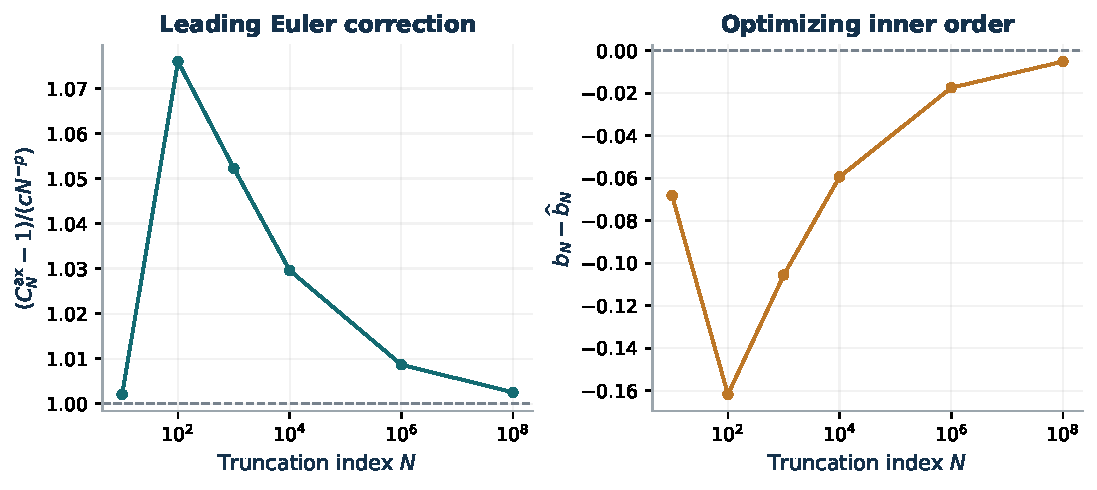
\includegraphics[width=\textwidth]{figures/euler_axis_asymptotics.pdf}
\caption{The optimized axis remainder approaches the proved leading
law, while the inner-order displacement tends to zero. The coefficient
in its finer inverse-logarithmic expansion is large, so moderate
indices need not display the final second-scale amplitude accurately.}
\label{fig:euler-axis}
\end{figure}

The second Euler scale deserves particular care: the proved
coefficient $T(B_0)\approx-2098.43$ makes the approach to its leading
amplitude slow. The data at $N\leq10^8$ are consistent with the first
asymptotic law; they are not a useful basis for fitting the much more
delicate next coefficient. The asymptotic proof identifies that
coefficient through a Mellin integral and uniform domination.

To resolve this slow approach numerically, the additional script
\nolinkurl{code/transition_remainder_diagnostics.py} evaluates the
positive Taylor remainder $\varepsilon_N(\widehat b_N)$ after dividing
by the gamma density at $t=\tfrac12\log N$. It forms no array of
length $N$ and uses stable exponential and hypergeometric remainders.
Define the dimensionless diagnostic
\[
 Q_N=\frac{\varepsilon_N(\widehat b_N)}
              {D_0N^{-\mu}/\sqrt{\log N}}.
\]
The theorem gives $Q_N\to1$ and
$(\log N)(Q_N-1)\to T(B_0)$. The following 75-digit quadratures
show how late these limits become numerically visible.

\begin{table}[htbp]
\centering
\begin{tabular}{rrr}
\toprule
$\log_{10}N$ & $Q_N$ & $(\log N)(Q_N-1)$\\
\midrule
8 & 0.1389757434 & $-15.860653$\\
100 & 0.3477552643 & $-150.184901$\\
1000 & 0.6776397628 & $-742.261877$\\
10000 & 0.9271461038 & $-1677.522954$\\
100000 & 0.9911352486 & $-2041.184436$\\
1000000 & 0.9990912540 & $-2092.464968$\\
\midrule
Proved limit & 1 & $-2098.428735$\\
\bottomrule
\end{tabular}
\caption{Transition-remainder diagnostics at the leading center
$\widehat b_N$. These evaluate the positive remainder at the stated
center. Large exponents are handled through
logarithms and normalized quadrature.}
\label{tab:transition-diagnostics}
\end{table}

At $N=10^8$, an independent direct-axis calculation minus the exact
first Taylor terms agrees with this normalized remainder to relative
error below $10^{-34}$. This is a numerical cross-check of the
implementation, not an interval certificate for the displayed
quadratures. The slow approach reinforces the need for the analytic
proof of the second scale.

\subsection{Pointwise kernel and inverse-series checks}

The kernel calculations solve the two stationary equations in the
scaled coordinates $(c,y)=(Nr,y)$ with 85-digit arithmetic.
At $N=2$ the exact certificate independently proves global optimality.
For other particular finite indices the table records stationary
candidates; the article's global uniqueness theorem is eventual.

\begin{table}[htbp]
\centering
\begin{tabular}{rrrr}
\toprule
$N$ & $Nr$ & $y$ & Stationary kernel value\\
\midrule
2 & 1.7045169541 & 0.2527026784 & 1.1189386860\\
4 & 2.3345294376 & 0.2084961852 & 1.0878146577\\
10 & 3.0411292987 & 0.1758872724 & 1.0689106048\\
100 & 3.8193399906 & 0.1489190557 & 1.0555582496\\
10000 & 3.9397958507 & 0.1453408168 & 1.0538792067\\
\bottomrule
\end{tabular}
\caption{Stationary-kernel diagnostics from the explicit rational
kernel, distinct from the order-averaged constants.}
\label{tab:kernel-diagnostics}
\end{table}

\begin{figure}[htbp]
\centering
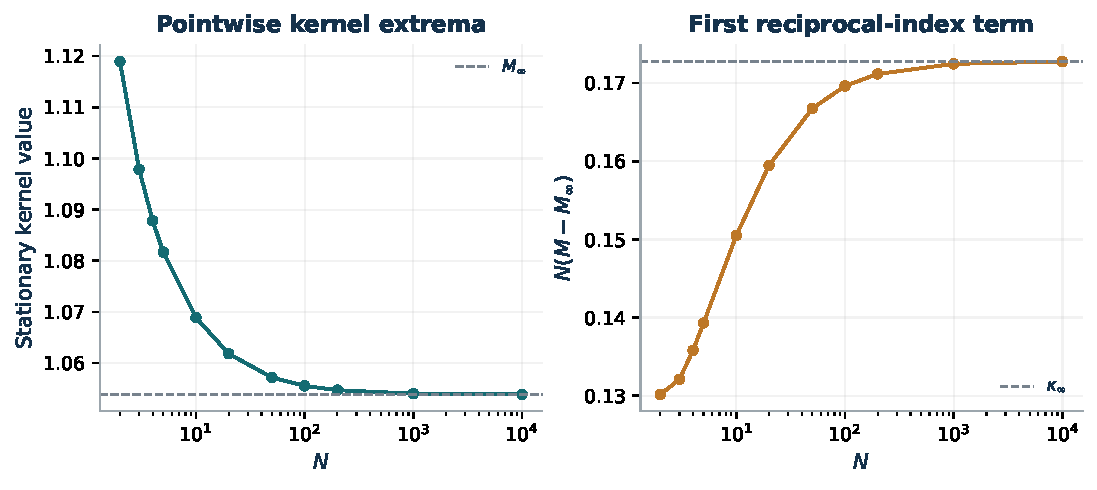
\includegraphics[width=\textwidth]{figures/kernel_limit.pdf}
\caption{Numerical stationary values and their first scaled excess.
The dashed levels are the analytically characterized $M_\infty$ and
$\kappa_\infty$. The proof of convergence covers all global maximizers
and does not depend on this stationary-point computation.}
\label{fig:kernel-limit}
\end{figure}

The inverse-series diagnostics use 360-digit arithmetic for
$A=1.1,2,4,10$ through index 240. Direct Stirling polynomial evaluation
and the independent coefficient recurrence agree to more than 150
relative decimal digits in every tested case. The record also compares
the exact barrier factorization at separate points, the first two
coefficient models, the boundary sums, and the renormalized derivative
sum. An error estimate involving a potentially vanishing cosine is
always displayed in additive normalized form.

\begin{figure}[htbp]
\centering
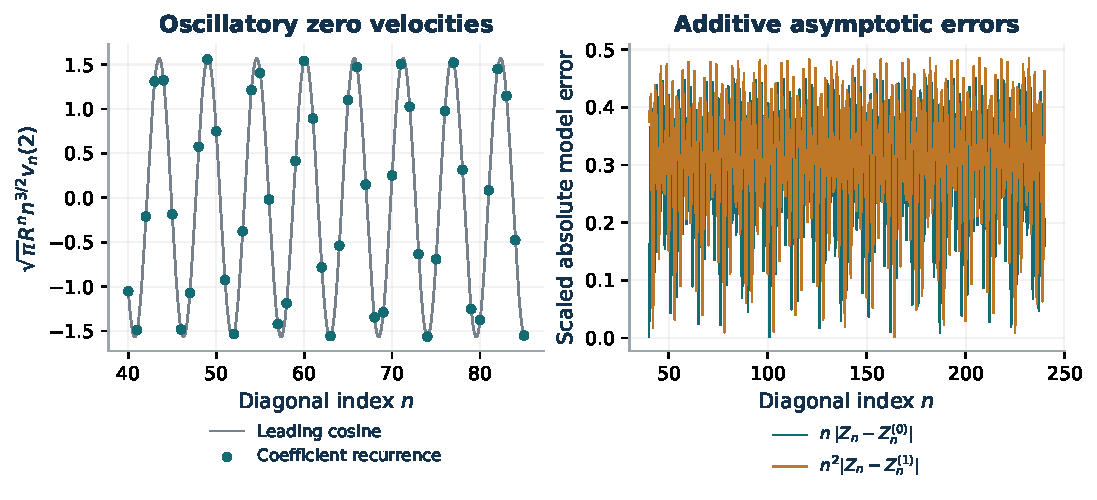
\includegraphics[width=\textwidth]{figures/harmonic_velocity_asymptotics.pdf}
\caption{At $A=2$, coefficients from an independent recurrence follow
the proved oscillatory phase. The right panel plots the errors after
the scalings predicted by the leading and corrected additive
asymptotics. These are finite numerical diagnostics of formulas whose
sheet selection and transfer hypotheses are proved analytically.}
\label{fig:harmonic-velocities}
\end{figure}

\subsection{Lambert roots at the bulk and at both endpoints}

For degrees 12, 30, and 60, the script
\nolinkurl{code/compute_bulk_root_examples.py} isolates every real root
of the exact rational polynomial by symbolic rational interval
arithmetic. Each positive-root interval has width at most $10^{-14}$;
all intervals have multiplicity one. Their midpoints are used only for
plotting. The distribution function is compared with the exact angle
law, and scaled polynomials are compared with the Bessel limit.

\begin{figure}[htbp]
\centering
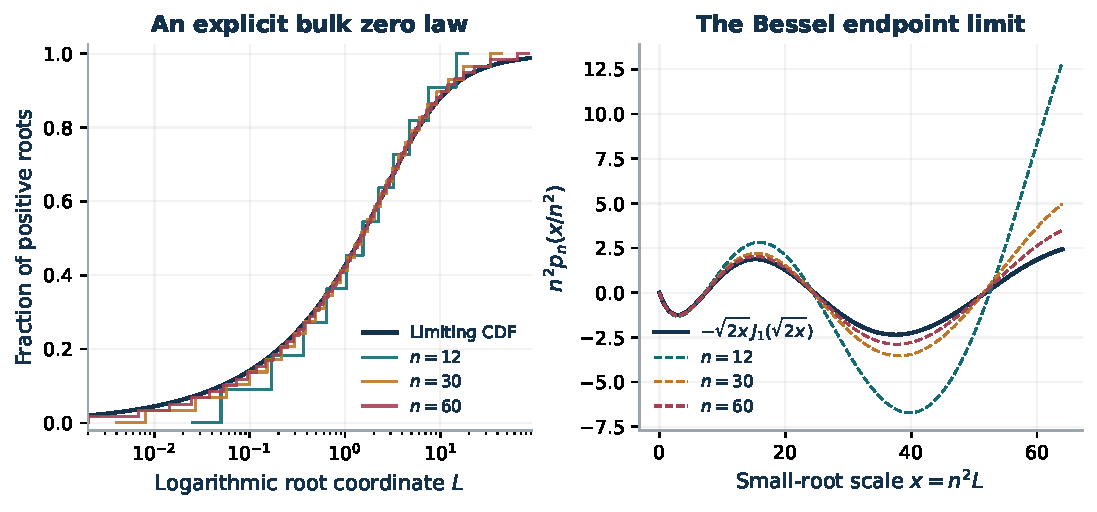
\includegraphics[width=\textwidth]{figures/lambert_bulk_and_bessel.pdf}
\caption{Left: finite positive-root distribution functions, based on
exact rational isolation, approach $\theta(L)/\pi$. Right: the
polynomial scaling at the small-root endpoint approaches the entire
Bessel function in \cref{thm:bessel-edge}. The logarithmic axis on
the left makes both endpoint regions visible.}
\label{fig:bulk-bessel}
\end{figure}

At the opposite endpoint, high-precision evaluation of the reciprocal
polynomial avoids its very large leading powers. The root diagnostics
cover 45 combinations of fixed $j,k$ and $64\leq n\leq1024$.
For $j=k=1$, define
\[
 B_n=n\bigl(X_{n,1,1}-n-\log n-\gamma\bigr),\qquad
 D_n=n^2\bigl(X_{n,1,1}-n-\log n-\gamma-C_0/n\bigr),
\]
where $C_0=-\tfrac32-\zeta(2)-\zeta(3)$.
The next table compares these quantities with their proved limits.

\begin{table}[htbp]
\centering
\begin{tabular}{rrr}
\toprule
$n$ & $B_n$ & $D_n$\\
\midrule
64 & $-4.25307307280$ & 6.01074542118\\
128 & $-4.29945689430$ & 6.08436169117\\
256 & $-4.32307710966$ & 6.12194824995\\
512 & $-4.33499694535$ & 6.14094062226\\
1024 & $-4.34098463490$ & 6.15048715477\\
\midrule
Proved limit & $-4.34699097001$ & 6.16006747240\\
\bottomrule
\end{tabular}
\caption{Largest-root diagnostics. The limit constants come from
exact symbolic formulas and the all-orders theorem.}
\label{tab:cohen-diagnostics}
\end{table}

\begin{figure}[htbp]
\centering
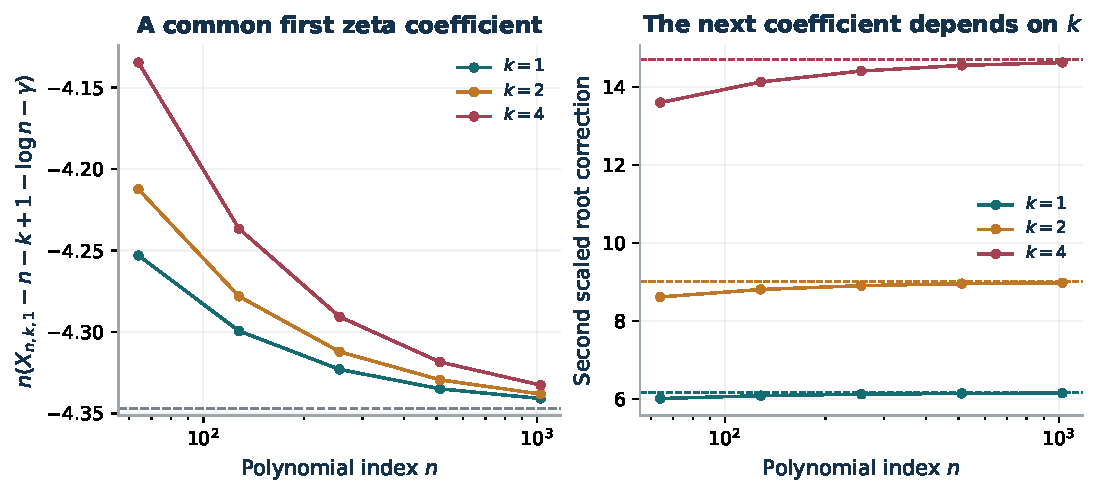
\includegraphics[width=\textwidth]{figures/cohen_extreme_root_coefficients.pdf}
\caption{The first largest-root correction is independent of $k$.
The next one is affine in $k-1$, with the exact expression proved in
\cref{sec:cohen-edges}; its respective limiting levels are dashed.
The numerical root residuals are separate from the analytic root
ordering and remainder proof.}
\label{fig:cohen-coefficients}
\end{figure}

The file \nolinkurl{data/figure_samples.json} also records finite
tests of the newly proposed indexed bulk-phase formula in
\cref{conj:bulk-quantization}. That conjecture is deliberately kept
out of every theorem dependency.

\subsection{Rebuilding and rechecking the package}

The main source is supplied both as \nolinkurl{article.tex} and as
modular sections with \nolinkurl{main.tex}. Run
\nolinkurl{python3 code/assemble_article.py} after editing modules,
then \nolinkurl{latexmk -pdf -halt-on-error article.tex}.
The file \nolinkurl{code/reproduce.py} replays the exact checks by
default; optional flags replay the more expensive diagnostics and
figures. A plain-text readme lists the individual commands and the
versions used. All scripts operate on local files and require no
repository write access or network connection.

The provenance directory pins the source revision and gives Git blob
hashes for retrieved material. A package checksum manifest records the
delivered files. The PDF was compiled from the supplied consolidated
TeX and visually checked after rendering, with particular attention to
long formulas, tables, cross-references, and the distinction between
the proved limits and finite diagnostics.
